% F043: equivalent vertical translation and horizontal compression of ln(x).
\begin{minipage}{.94\linewidth}\centering
  \definecolor{F043logbase}{RGB}{197,74,60}
  \definecolor{F043lognew}{RGB}{32,100,180}
  \definecolor{F043logguide}{RGB}{0,120,100}
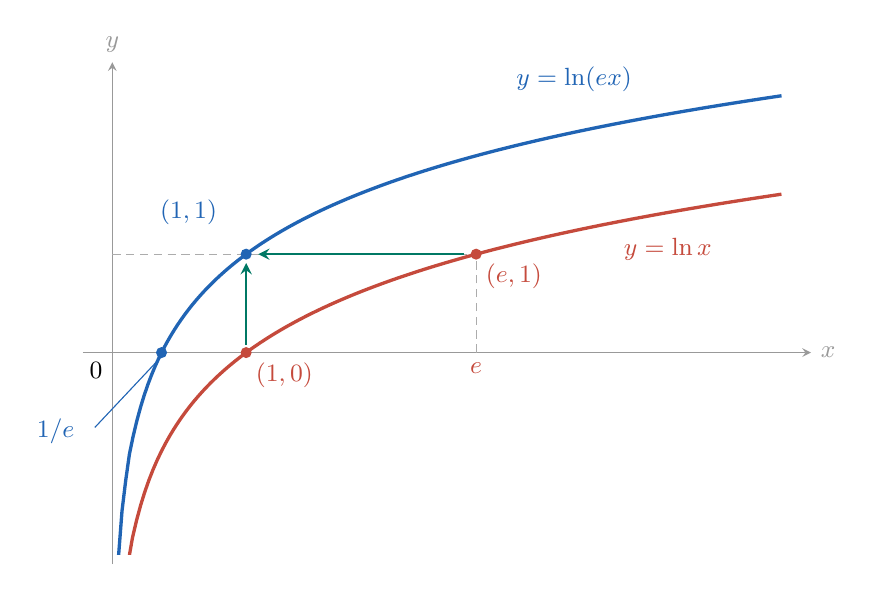
\begin{tikzpicture}[x=1.70cm,y=1.25cm,>=stealth,font=\small]
  \draw[->,gray!80] (-0.22,0)--(5.22,0) node[right] {$x$};
  \draw[->,gray!80] (0,-2.15)--(0,2.95) node[above] {$y$};
  \node[below left] at (0,0) {$0$};
  \begin{scope}
    \clip (0,-2.05) rectangle (5.05,2.85);
    \draw[F043logbase,very thick,domain=0.12:5,samples=160] plot (\x,{ln(\x)});
    \draw[F043lognew,very thick,domain=0.045:5,samples=180] plot (\x,{ln(\x)+1});
  \end{scope}
  \draw[gray!65,densely dashed] (0,1)--(2.718281828,1);
  \draw[gray!65,densely dashed] (2.718281828,0)--(2.718281828,1);
  % Keep the two correspondences visible; put their explanations below the plot.
  \draw[->,F043logguide,thick] (1,0.08)--(1,0.91);
  \draw[->,F043logguide,thick] (2.63,1)--(1.09,1);
  \fill[F043logbase] (1,0) circle (2pt);
  \fill[F043logbase] (2.718281828,1) circle (2pt);
  \fill[F043lognew] (1,1) circle (2pt);
  \fill[F043lognew] (0.367879441,0) circle (2pt);
  \node[F043logbase,below right] at (1,0) {$(1,0)$};
  \node[F043lognew,above left=7pt] at (1,1) {$(1,1)$};
  \node[F043logbase,below right] at (2.718281828,1) {$(e,1)$};
  \node[F043logbase,below] at (2.718281828,0) {$e$};
  \draw[F043lognew,thin] (0.367879441,-0.04)--(-0.13,-0.76);
  \node[F043lognew,anchor=east] at (-0.21,-0.80) {$1/e$};
  \node[F043lognew] at (3.45,2.78) {$y=\ln(ex)$};
  \node[F043logbase] at (4.15,1.05) {$y=\ln x$};
\end{tikzpicture}
\par\smallskip
{\small\textcolor{F043logguide}{竖直箭头：上移 $1$，$(1,0)\to(1,1)$。}}\par
{\small\textcolor{F043logguide}{水平箭头：横坐标变为原来的 $1/e$，$(e,1)\to(1,1)$。}}\par
\end{minipage}
